\documentclass[a4paper,11pt]{article}
\usepackage[utf8]{inputenc} 
\usepackage[MeX]{polski}
\usepackage{nicefrac}
\usepackage[usenames, dvipsnames]{xcolor}
\usepackage{amsmath}
\usepackage{amssymb}
\usepackage{color, colortbl}
\usepackage{graphicx,color}
\usepackage{indentfirst}
\usepackage{array,booktabs,wrapfig} % http://ctan.org/pkg/booktabs
\usepackage[a4paper,top=1.5cm,bottom=2cm,left=2.0cm,right=2.0cm]{geometry}
\usepackage{hhline}
\usepackage[pdftex,hyperfootnotes=false,pdfborder={0 0 0}]{hyperref}

\usepackage{array}
\newcolumntype{L}[1]{>{\raggedright\let\newline\\\arraybackslash\hspace{0pt}}m{#1}}
\newcolumntype{C}[1]{>{\centering\let\newline\\\arraybackslash\hspace{0pt}}m{#1}}
\newcolumntype{R}[1]{>{\raggedleft\let\newline\\\arraybackslash\hspace{0pt}}m{#1}}

\definecolor{darkblue}{rgb}{0.0, 0.0, 0.55}
\definecolor{darkred}{rgb}{0.5, 0.0, 0.0}
\definecolor{darkgreen}{rgb}{0.0, 0.5, 0.0}

% ----------- Custom commands -----------
\newcommand{\myBoldBlue}[1]{\textbf{\textcolor{darkblue}{#1}}}
\newcommand{\myColorBox}[2]{\colorbox{#1}{\begin{minipage}[t]{\textwidth}#2\end{minipage}}}
\newcommand{\myNiceCBox}[2]{\colorbox{#1}{\strut\makebox{#2}}}
\newcommand{\footref}[1]{%
	$^{\ref{#1}}$%
}
% ---------------------------------------
\newcommand{\myHeaderCellColor}{\cellcolor{black!10}}

% Do rysowania wektorów o rozmiarze dwa
\newcommand{\myVectorC}[2]{\begin{bmatrix}#1\\#2\end{bmatrix}}
\newcommand{\myVectorR}[2]{\begin{bmatrix}#1&#2\end{bmatrix}}
\newcommand{\myDotProduct}[2]{\langle #1, #2\rangle}

\pagestyle{empty}

\newcommand{\emptybox}[2][\textwidth]{%
	\begingroup
	\setlength{\fboxsep}{-\fboxrule}%
	\noindent\framebox[#1]{\rule{0pt}{#2}}%
	\endgroup
}



% Definiowanie zmiennych w Latexu
% \def \variable {Something that's better to use as a variable}

\newcommand{\myEmptySpace}{\hspace{0.8cm}}

\pagenumbering{gobble}

\begin{document}
\title{{\large SkaiWD -- Laboratorium 4}\\\textbf{PCA -- przykład}}
%\author{Iwo Błądek}
\date{}
\maketitle
\vspace{-1cm}

\def \myZadanieOdstep {1cm}
\newcounter{myTaskNumber}[section]
\newcommand{\theMyTaskNumber}{\stepcounter{myTaskNumber}\arabic{myTaskNumber}}
\newcommand{\theMySectNumber}{\arabic{section}}


\noindent\begin{minipage}[t]{0.3\textwidth}
\noindent\textbf{Dane:}\medskip\\
\begin{tabular}{l|r|r|}
%\cline{2-3}
\hhline{|~|-|-|}
& $x_1$\myHeaderCellColor & $x_2$\myHeaderCellColor\\\cline{2-3}
&-2&-2\\\cline{2-3}
&-1&0\\\cline{2-3}
&0&1\\\cline{2-3}
&1&-1\\\cline{2-3}
&2&2\\\hline
%&-1&-1\\\cline{2-3}
%&0&1\\\cline{2-3}
%&1&2\\\cline{2-3}
%&2&0\\\cline{2-3}
%&3&3\\\hline
\multicolumn{1}{|l|}{avg\myHeaderCellColor} &0 &0 \\\hline
\end{tabular}
\end{minipage}
%
%\begin{minipage}[t]{0.3\textwidth}
%\noindent\textbf{Dane wycentrowane:}\medskip\\
%\begin{tabular}{|r|r|}
%\hline
%$x_1$\myHeaderCellColor & $x_2$\myHeaderCellColor\\\hline
%\myEmptySpace&\myEmptySpace\\\hline
%\myEmptySpace&\myEmptySpace\\\hline
%\myEmptySpace&\myEmptySpace\\\hline
%\myEmptySpace&\myEmptySpace\\\hline
%\myEmptySpace&\myEmptySpace\\\hline
%\end{tabular}
%\end{minipage}
%
\begin{minipage}[t]{0.3\textwidth}
\noindent\textbf{Macierz kowariancji:}\medskip\\
\begin{tabular}{l|r|r|}
%\cline{2-3}
\hhline{|~|-|-|}
& $x_1$\myHeaderCellColor & $x_2$\myHeaderCellColor\\\hline
\multicolumn{1}{|l|}{$x_1$\myHeaderCellColor} & 2.50 & 1.75 \\\hline
\multicolumn{1}{|l|}{$x_2$\myHeaderCellColor} & 1.75 & 2.50 \\\hline
\end{tabular}
\end{minipage}
%
\begin{minipage}[t]{0.45\textwidth}
	\noindent\textbf{Wykres:}\\\vspace{-0.1cm}
	\hspace{-0.85cm}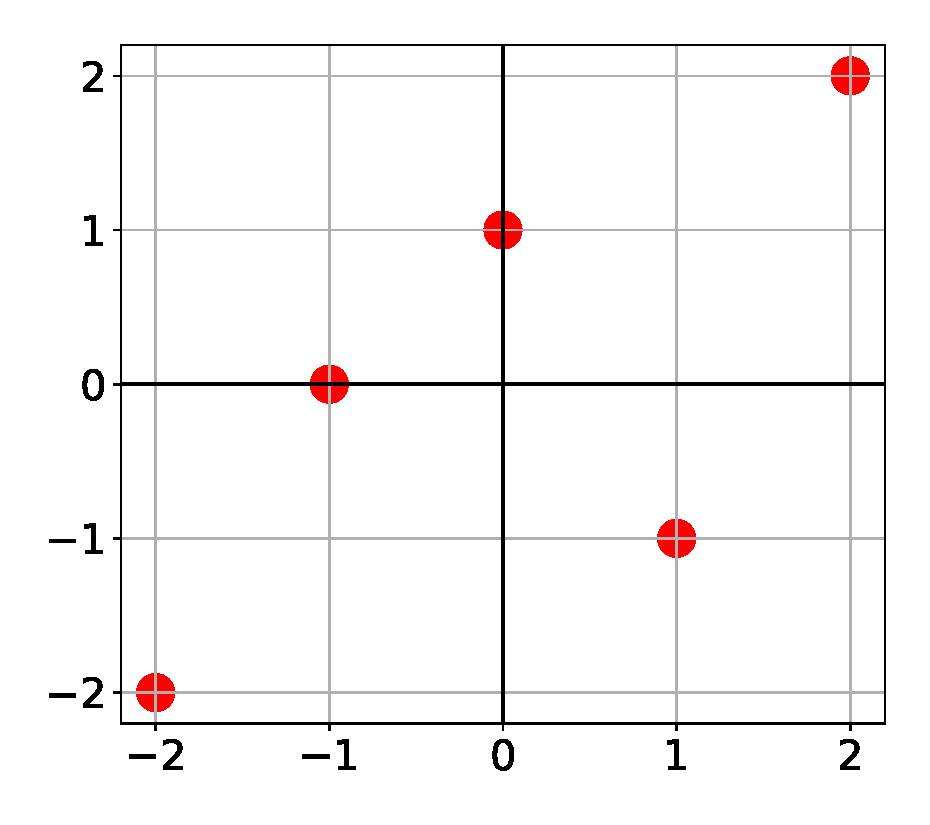
\includegraphics[width=0.9\textwidth]{img/chart_pca_clear_x.pdf}
\end{minipage}



\noindent\textbf{Miejsce na obliczenia:}\medskip\\
Macierz kowariancji X: $Cov_{X} = \frac{1}{4}X^{T}X$ \vspace{0.2cm} \\
Wartości własne $Cov_{X}$: $(2.5 - \lambda)^2 - 1.75^2 = 0 \iff \lambda^2 - 5\lambda + \frac{51}{16}=0 \iff
\lambda = 4.25 \lor \lambda =0.75$ \vspace{0.2cm} \\
Pierwszy wektor własny $k_1$: $-1.75x_1 + 1.75x_2 = 0 \land 1.75x_1 - 1.75x_2 = 0 \iff x_1=x_2$ \vspace{0.2cm} \\
Drugi wektor własny $k_2$: $1.75x_1 + 1.75x_2 = 0 \land 1.75x_1 + 1.75x_2 = 0 \iff x_1=-x_2$ 
%\emptybox[\linewidth]{5cm}


\bigskip
\noindent\textbf{Posortowane malejąco wartości i wektory własne (znormalizowane):}\medskip\\
\begin{minipage}{0.2\textwidth}
$\lambda_1 = \underline{4.25}$\bigskip\\
    $k_1 = \begin{bmatrix} \tfrac{\sqrt{2}}{2} \vspace{0.1cm} \\ \tfrac{\sqrt{2}}{2}\end{bmatrix}$
\end{minipage}
\hspace{0.05\textwidth}
\begin{minipage}{0.2\textwidth}
	$\lambda_2 = \underline{0.75}$\bigskip\\
    $k_2 = \begin{bmatrix} - \tfrac{\sqrt{2}}{2} \vspace{0.1cm} \\ \tfrac{\sqrt{2}}{2}\end{bmatrix}$
\end{minipage}
\hspace{0.05\textwidth}
\begin{minipage}{0.3\textwidth}
	$K = \begin{bmatrix}
	\tfrac{\sqrt{2}}{2}{} & - \tfrac{\sqrt{2}}{2} \vspace{0.3cm}\\
	\tfrac{\sqrt{2}}{2} & \tfrac{\sqrt{2}}{2}
	\end{bmatrix}$
\end{minipage}


\vspace{1cm}


\noindent\begin{minipage}[t]{0.3\textwidth}
	\noindent\textbf{Dane po PCA:}\medskip\\
	$Y = XK =$
	\begin{tabular}{|c|c|}
		\hline
		$y_1$\myHeaderCellColor & $y_2$\myHeaderCellColor  \\\hline
        $-2\sqrt{2}$ & 0 \\\hline
        $-\tfrac{\sqrt{2}}{2}$ & $\tfrac{\sqrt{2}}{2}$ \\\hline
        $\tfrac{\sqrt{2}}{2} $ &  $\tfrac{\sqrt{2}}{2}$ \\\hline
        $0$ & $-\sqrt{2}$ \\\hline
        $2\sqrt{2}$ & 0 \\\hline
	\end{tabular}

	\bigskip
	\bigskip

    $y_1(x_1, x_2) = \underline{k_{11}}~x_1 + \underline{k_{12}}~x_2$\smallskip\\
    $y_2(x_1, x_2) = \underline{k_{21}}~x_1 + \underline{k_{22}}~x_2$

\end{minipage}
%
\begin{minipage}[t]{0.3\textwidth}
	\noindent\textbf{Macierz kowariancji:}\medskip\\
	\begin{tabular}{l|r|r|}
%		\cline{2-3}
		\hhline{|~|-|-|}
		& $y_1$\myHeaderCellColor & $y_2$\myHeaderCellColor\\\hline
		\multicolumn{1}{|l|}{$y_1$\myHeaderCellColor} & 4.25 & 0.00 \\\hline
		\multicolumn{1}{|l|}{$y_2$\myHeaderCellColor} & 0.00 & 0.75 \\\hline
	\end{tabular}
\end{minipage}
%
\begin{minipage}[t]{0.45\textwidth}
	\noindent\textbf{Wykres:}\\\vspace{-0.1cm}
	\hspace{-0.85cm}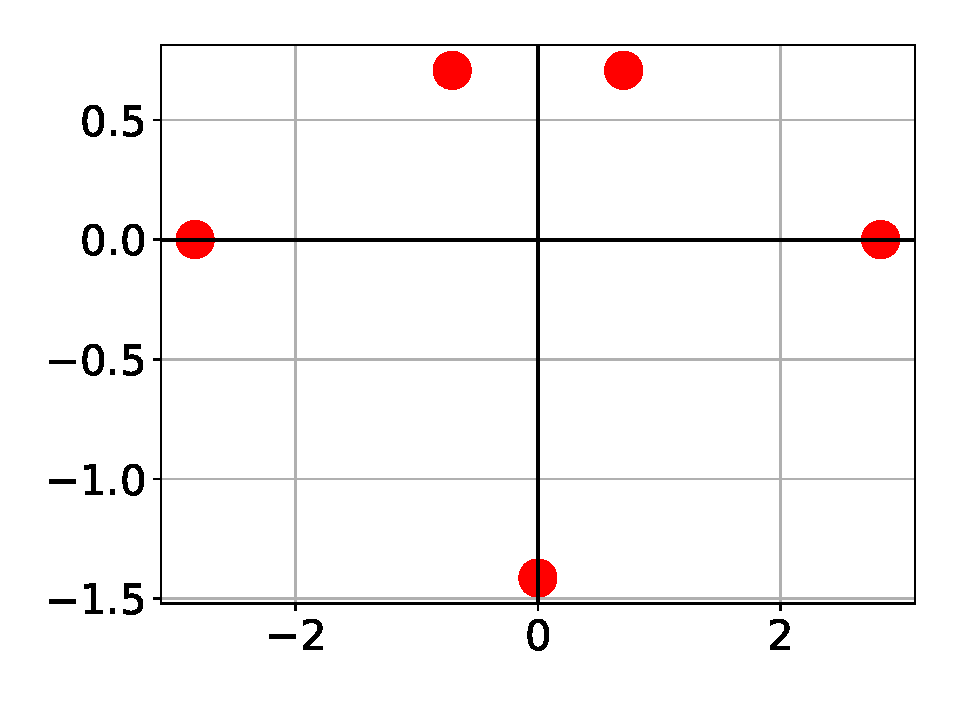
\includegraphics[width=0.9\textwidth]{img/chart_pca_clear_y.pdf}
\end{minipage}

\end{document}
